%!TEX root = ../main.tex
After developing the initial version of TAPS, I realised that the solution was not broad enough in terms of what type of network it could accurately translate. The type of network that is possible to translate with the initial version of TAPS, is a network that does not keep internal states between clock cycles.
In the seven-segment example, no internal results have any influence on the result from other clock cycles, and therefore it can be correctly translated using the structures described in the previous chapters.
However, the original TAPS system was unable to generate semantically equivalent \cspm{} code from networks where the results depend on the internal state of the network. Examples of such networks include the \texttt{addone} example from \cite{smeil}.\\

The \texttt{addone} network is a simple cyclic network that consists of two processes communicating with each other. The SMEIL code for this example can be seen in Listing \ref{lst:addone_smeil_example}. The \texttt{add} process receives a value and increments it by a constant parameter. The \texttt{id} process receives the value and passes it along on its output bus.
An illustration of the network can be seen in Figure \ref{fig:addone_unclocked}.\\
\begin{figure}
    \centering
    \begin{tikzpicture}
       \node[mycircle] (add) {$add$};
       \node[mycircle] (id) [right = 3cm of add] {$id$};

       \path[myarrow, smooth, bend right=30]
       (add) edge node {} (id);
       \path[myarrow, smooth, bend right=30]
       (id) edge node {} (add);

       \node[align=center, below, text width=1.7cm] at (2.2,1.3){\footnotesize\texttt{channel d}};
       \node[align=center, below, text width=1.7cm] at (2.2,-0.9){\footnotesize\texttt{channel c}};
   \end{tikzpicture}
    \caption{The \texttt{addone} network consists of two proceses that communicate to each other on channel \texttt{c} and \texttt{d}.}
    \label{fig:addone_unclocked}
\end{figure}

As presented in Chapter \ref{chap:design}, all possible communication combinations are represented in the generated \cspm{} code, however, the generated \cspm{} processes are not recursing, and so only one cycle of the loop is simulated in the \texttt{addone} example. This means that if the network was provided with an input that, after several clock cycles, resulted in a failure, this would not be caught by FDR4 because the \cspm{} code only represents one clock cycle. It was, therefore, necessary to extend TAPS so that network with internal states can be verified.\\
\begin{listing}
\begin{minted}{smeil_lexer.py:SMEILLexer -x}
proc add (in inbus, const constant)
    bus outbus {
        val: u4 = 0 range 0 to 10;
    };
{
    outbus.val = inbus.val + constant;
}

proc id (in inbus)
    bus outbus {
        val: u4 = 0 range 0 to 10;
    };
    var from_add: u4 range 0 to 10;
{
    from_add = inbus.val;
    outbus.val = from_add;
}


network addone_network ()
{
    instance id of id(add.outbus);
    instance add of add(id.outbus, constant: 1);
}
\end{minted}
\caption{The simulated SMEIL network \texttt{addone\_network} with two processes. The example is similar with the addone example in \cite{smeil}. The }
\label{lst:addone_smeil_example}
\end{listing}

The purpose of the initial design of TAPS was to model a synchronous network in \cspm{} without having to model a global synchronous clock. As described in Chapter \ref{chap:background}, the results from the master's thesis \textit{Generation of FPGA Hardware
Specifications from PyCSP Networks}~\cite{Skaarup14} by E. Skaarup and A. Frisch, established how much the complexity of the network would increase when trying to model this in CSP.
However, the \texttt{addone} example shows that it is necessary to extend TAPS to model a global synchronous structure in \cspm{}. As Skaarup and Frisch already learned, enforcing a global synchronous model onto CSP is not trivial, and even simple networks quickly become very complex. The reason for even considering implementing this structure in spite of the results from \cite{Skaarup14}, is that TAPS will auto-generate the \cspm{} code and therefore the complexity and size of the corresponding \cspm{} network is less of an issue. However, the extra complexity might become a problem when verifying with FDR4. It is possible that the added complexity of the network increases the requirements for FDR4, and that the size of problems verifiable with FDR4, becomes smaller with this solution. \\

In this chapter, I will introduce the approach for extending TAPS to translate clocked systems.
\section{Global Synchronisation}
In order to verify networks for more than one clock cycle, it is necessary to translate the SMEIL processes to recursive \cspm{} processes. As explained in the CSP background section in Chapter \ref{chap:background}, these types of processes do not terminate with \texttt{SKIP} but will behave as itself forever, unless the network informs otherwise.
An example of this can be seen in Listing \ref{lst:cspm_recursion}.
\begin{listing}
\begin{minted}{cspm_lexer.py:CSPmLexer -x}
Init = d ! 1 -> Inc(1)
Inc(x) = d ! (x+1) -> Inc(x+1)
\end{minted}
\caption{Example of the a recursive \cspm{} process that is initialised by the \texttt{Init} process.}
\label{lst:cspm_recursion}
\end{listing}

An actual SME process will never terminate, but it is of course not possible to simulate endless runtime, so when simulating the SMEIL network the developer indicates the number of clock cycles to simulate. The results of the simulation can be seen as a snapshot of the process trace. The SMEIL simulation consists of a finite number of clock cycles and it is not possible to verify an infinite state space with FDR4, therefore, it is necessary to introduce process termination to the translation, even though this is not the reality of actual hardware. \\

In Listing \ref{lst:cspm_recursion}, process \texttt{Inc} performs an endless loop with no option to terminate. As previously mentioned, it is important to limit the range of values for FDR4 to verify, in order to avoid running out of space. If the example in Listing \ref{lst:cspm_recursion} was verified with FDR4, it would eventually run out of space. It is therefore crucial to model a structure that can drive the network synchronisation, and that can ensure that the processes terminate at a specified time. This structure is represented by a \texttt{Clock} process added to the generated network in \cspm{}. The \texttt{Clock} process drives the network for a specific number of clock cycles and then terminates, causing all other processes to do the same. \\

It is, of course, still necessary for the new version of TAPS to model a \cspm{} network that reflects the SME model, and therefore it must adhere to the SME model structure. To model the global synchronicity in \cspm{}, it is necessary to enforce a synchronising event. This synchronicity can be emulated by having a \texttt{sync} channel, where all processes synchronise and thus they can emulate rising and falling clock signals. All clocked processes in the network will synchronise on the \texttt{sync} channel, and as previously introduced, when two processes are synchronised on a channel, they must agree on communication before any process can continue. The same \texttt{sync} channel is used for syncronising read as well as write, thus all processes syncronise on the \texttt{sync} channel before they read and before they write.
The \texttt{Clock} process is also synchronising on the \texttt{sync} channel, so when the specified number of clock cycles has passed, the \texttt{Clock} process terminates.
This means that none of the other processes will be able to synchronise on the \texttt{sync} channel because all processes must synchronise together. They will instead behave as \texttt{SKIP} and so the system terminates successfully.\\

It is possible to design the \texttt{Clock} process to send values to each process, so that the process itself decides to terminate or continue, based on the value received. However, this would increase the complexity of the processes. The \texttt{Clock} process is instead designed to perform the \texttt{sync} event twice, one for read and one for write, for each clock cycle, and then recurse. In Listing \ref{lst:clock_process}, the \cspm{} code for a \texttt{Clock} process can be seen. The \texttt{Clock} process is instantiated with a start value and the desired number of clock cycles, so for each recursion, the internal value is incremented by one. By using pattern matching, the internal value of the \texttt{Clock} process is checked against the number of desired clock cycles, and if it is equal, the process terminates by \texttt{SKIP}. When the \texttt{Clock} process has terminated, all other processes will terminate as well.
\begin{listing}
\begin{minted}{cspm_lexer.py:CSPmLexer -x}
Clock(10) = SKIP
Clock(n) =  sync -> sync -> Clock(n+1)
\end{minted}
\caption{Example of a \texttt{Clock} process that runs for 10 clock cycles before terminating. }
\label{lst:clock_process}
\end{listing}

\section{Clocked Processes}
All clocked processes must synchronise on the same \texttt{sync} channel as the \texttt{Clock} process described above. Each process must synchronise on this channel twice in each clock cycle, and then recurse. To ensure the SME model structure is kept intact, the clocked processes are still defined with the \texttt{let within} structure, but the read must happen inside the process itself. A read can be performed in every clock cycle and therefore the read cannot happen in the surrounding network as in the initial version of TAPS.\\

As explained in Chapter \ref{chap:design}, the initial version of TAPS performs reads for each process outside of the process itself, which simplifies the translation, but it is not completely consistent with the SME model. Listing \ref{lst:cspm_input_values_examples} in Chapter \ref{chap:design} introduces three different methods for translating the input buses from SMEIL to \cspm{}. The method that matches the SME model best, is the method in Listing \ref{lst:cspm_channel_reads_input}, where the process parameter is a placeholder for the channel name and so the process can read the value directly from the placeholder. Because a clocked process can read an input in each clock cycle, the read must be within the process recursion. Therefore the solution used in the initial version of TAPS cannot be used in the clocked version, so the method used in the clocked version of TAPS is the method from Listing \ref{lst:cspm_channel_reads_input}.\\

To ensure the synchronicity of the network, each process must synchronise before a read and before a write and so a simplified process structure looks like this:
\begin{minted}{cspm_lexer.py:CSPmLexer -x}
P = sync -> read_channel ? val -> sync -> compute -> write_channel ! val -> P
\end{minted}
This is, of course, not including computation, so after the second synchronisation the process can include a \texttt{let within} structure with all computations and writes.
\begin{minted}{cspm_lexer.py:CSPmLexer -x}
P = sync ->
    read_channel ? val ->
    sync ->
    let
        compute
    within
        write_channel ! val -> P
\end{minted}
This \texttt{let within} structure is only necessary if the process is actually performing computation. The \texttt{id} process in Listing \ref{lst:addone_smeil_example} does not compute but only reads and writes, and therefore TAPS must not include the \texttt{let within} structure, because FDR4 will fail if an empty \texttt{let} is included. Similarly, not all processes both reads and writes, and therefore TAPS has to adapt the process structure to accommodate this. It is, however, still possible to keep the overall structure of the process even though a process does not read or write. A process that does not read can look like this:
\begin{minted}{cspm_lexer.py:CSPmLexer -x}
P = sync ->
    sync ->
    let
        compute
    within
        write_channel ! val -> P
\end{minted}
The process synchronises twice in a row because it does not perform a read in the read phase and therefore it must wait to compute and write in the write phase. \\

Simple calculations in SMEIL can be included in-line with the read and the write. An example of this can be seen in the \texttt{add} process in Listing \ref{lst:addone_smeil_example} where \texttt{constant} is added to the input value and written to the output bus on the same line.
Listing \ref{lst:cspm_computation} shows two examples of dividing simple computation in \cspm{}.
As seen, the simple computation of the \texttt{add} process can trivially be included directly to the read or write.
However, to simplify its implementation, TAPS does not distinguish the generated code based on the complexity of expressions.
Therefore, these types of SMEIL structures will be divided into a separate read and write by TAPS.
This means that the example in Listing \ref{lst:cspm_computation_simple} will be fitted to the general solution that can be seen in Listing \ref{lst:cspm_computation_letwithin}, even though it is unnecessarily complex. As previously explained, this is one of the disadvantages of auto-generated code.\\
\begin{minipage}[t]{.98\linewidth}
    \centering
\begin{minipage}[t]{0.45\linewidth}
\begin{minted}[stripnl=false]{cspm_lexer.py:CSPmLexer -x}
P = read_channel ? val ->
    write_channel ! val + 1 -> P



\end{minted}
  \captionof{listing}{An example of an addition computation added directly to the \cspm{} write.}
  \label{lst:cspm_computation_simple}
\end{minipage}
\hspace{0.6cm}
\begin{minipage}[t]{0.45\linewidth}
\begin{minted}{cspm_lexer.py:CSPmLexer -x}
P = read_channel ? val ->
    let
        result = val + 1
    within
        write_channel ! result -> P
\end{minted}
\captionof{listing}{An example of an addition computation and a write separated by the \texttt{let within} structure.}
\label{lst:cspm_computation_letwithin}
\end{minipage}
\vspace{0.3cm}
\captionof{listing}{Examples of how a simple computation must adhere to the general translation structures in \cspm{}.}
\label{lst:cspm_computation}
\vspace{1cm}
\end{minipage}

In Listing \ref{lst:cspm_computation_letwithin}, the process first reads a value from \texttt{read\_channel}, then computes the result within the \texttt{let} section and then writes the result to \texttt{write\_channel} in the \texttt{within} section.
\section{Introducing Buffers}
As can be seen in Figure \ref{fig:addone_unclocked}, both the \texttt{id} process and the \texttt{add} process are both reading and writing. A problem occurs because they are both trying to read and write at the same time. It is clear that both processes cannot begin by reading, because no process has yet written anything for the other to read.
To solve this problem, TAPS defines a buffer structure for each SMEIL channel. A buffer is a process that stores data between clock cycles. The buffer first writes a value to a channel and then reads a value from a channel, all in one clock cycle. Thus, the buffer structure is the reverse of a 'normal' process, because it will write first and then read in a clock cycle. Figure \ref{fig:clock_cycle} illustrates the relation between a process and a buffer.\\

\begin{figure}
\centering
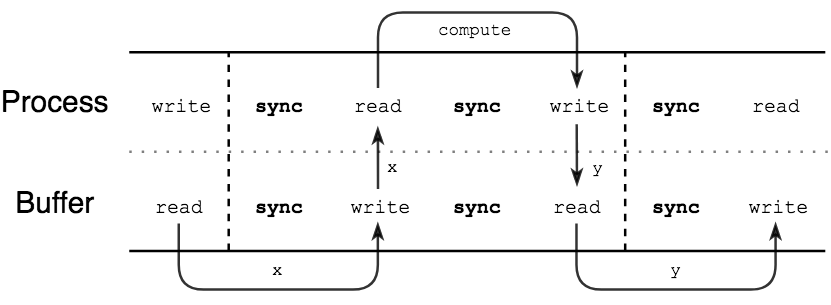
\includegraphics[width=0.75\textwidth]{./figures/clock_cycle_thesis.png}
\caption{Illustration of the relation between a process and a buffer. In one clock cycle the buffer writes a value which the process reads, and after the computation the process writes the value to the buffer which holds it for the next clock cycle.}
\label{fig:clock_cycle}
\end{figure}
The buffer solves the problem of initialising the network. Each buffer is instantiated with a value that the buffer writes to a channel from which a process can read. However, the initial value is only used to initialise the network. I refer to the initial value as a \textit{dummy value} which is determined as a value outside of the channel range so that the process is able to distinguish between the initial value and the actual network values.
It is, of course, not ideal to represent the dummy value as an integer. The dummy value must be outside the channel range, and therefore the channel range cannot represent the entire signed 32-bit representation that FDR4 support. Even though it is highly unlikely for a channel range to be this large, it is an unnecessary restriction. It is possible to define a data structure in \cspm{} that removes this restriction, for example by having the dummy value being represented by a boolean instead of an integer. This extended structure will increase the complexity of the communication structures, but it is simple to auto-generate.
In this thesis, the dummy value is represented by an integer value to simplify the examples.\\
% TODO: Is it clear that I am talking about the addone example here below?
The \texttt{add} process and the \texttt{id} process are both instantiated with a value, which is used instead of the initial dummy value from the buffer process. When the process encounters the dummy value, the process ignores it and continues with the value that the process was instantiated with instead. After the first clock cycle, the process loop will continue, and the communication will hold according to the SME model.\\

A clocked version of the \texttt{addone} network can be seen in Figure \ref{fig:addone_clocked}. The clocked \texttt{addone} network consists of four channels, two buffer read channels and two buffer write channels. A buffer process is defined for each original channel in the \texttt{addone} network. \\

\begin{figure}
\centering
\begin{tikzpicture}
\node[mycircle] (add) {$add$};
\node[mycircle] (id) [right = 4cm of add] {$id$};
\node[mycircle, semithick] (bufd) at (2.7, 1.7) {$Buf_d$};
\node[mycircle, semithick] (bufc) at (2.7, -1.5) {$Buf_c$};


\path[myarrow, smooth, bend right=25]
(add) edge node {} (bufc);



\path[myarrow, smooth, bend right=25]
(bufc) edge node {} (id);
\path[myarrow, smooth, bend right=25]
(id) edge node {} (bufd);


\path[myarrow, smooth, bend right=25]
(bufd) edge node {} (add);


\node[align=center, below, font=\footnotesize] at (1.5,1.2){\texttt{d\_write}};
\node[align=center, below, font=\footnotesize] at (3.8,1.2){\texttt{d\_read}};
\node[align=center, below, font=\footnotesize] at (1.5,-0.7){\texttt{c\_read}};
\node[align=center, below, font=\footnotesize] at (3.8,-0.7){\texttt{c\_write}};

\end{tikzpicture}
\caption{The clocked \texttt{addone} network has two proceses and two buffers, which ensure the global synchronicity.}
\label{fig:addone_clocked}
\end{figure}
\section{Buffer Structure}
The buffers are designed to adhere to different kinds of process behaviour, and therefore the structure becomes complex. However, the buffer structures are standardized, so that they can be used for all clocked SMEIL channels. Therefore the complexity is not an issue when auto-generating the buffer. A buffer must still comply with the synchronisation of the network, so a buffer is divided into a read and a write structure to simplify the buffer structure, and to comply with some of the requirements that the SME model sets for the processes, which will be explained below. \\

The buffer structure can be seen in Listing \ref{lst:buffer}.
A buffer writes first in a clock cycle. The \texttt{Write\_buf} is initialised and will behave according to the possible communication.\\

When a network is initialised, all processes will synchronise first and then the \texttt{Write\_buf} process will write its initial value to the corresponding channel. The write can be seen in Listing \ref{lst:buffer} in the \texttt{Writes\_buf} process. The reason for creating a separate process for the actual write event, is that the SME model specifies that several processes can read the same value from the buffer in the same clock cycle. It is therefore necessary to define a recursive structure that enables several buffer writes in the same clock cycle. The \texttt{Writes\_buf} process will write a value to the channel and then either write again or behave as the \texttt{Read\_buf} process.\\

If no processes are reading from the buffer, the buffer will not write, and instead behaves as the \texttt{Read\_buf} process. This can be seen as the external choice between the \texttt{Writes\_buf} process and the \texttt{Read\_buf} process, after the initial synchronisation in the \texttt{Write\_buf} process.
The last action before a process terminates will always be a write, which means that the buffer will read the value and then terminate. The buffer must have the choice to terminate after a read, otherwise, it would wait forever and FDR4 would fail. \\

It is defined in the SME model, that a buffer can never be written to twice in the same clock cycle. In the current version of SMEIL, this is not implemented, as several processes can write to the same bus within the same clock cycle. However, this is not an accurate solution and a check must be added in SMEIL to ensure that this never happens. To verify that two reads cannot happen in the same clock cycle, an extra assertion have been added to the buffer structure.
If more than one read can be performed by the \texttt{Read\_buf} process, the process behaves as the \texttt{STOP} process which indicates failure, and thus FDR4 would catch the failure when verifying the network.\\

The SME model requires that there are no values to be read from the buffer if no value was written to it. And therefore the buffer does not perform a write in a clock cycle if it did not read a value in the previous clock cycle. This can be seen in the \texttt{Read\_buf} process as the external choice between reading or synchronising and then recursing to the \texttt{Read\_buf} process again.\\

In the unlikely case that there are no writes to the buffer at all, the buffer must be able to terminate along with the rest of the processes and therefore the \texttt{Read\_buf} process also includes an external choice with \texttt{SKIP}.

\begin{listing}
\begin{minted}{cspm_lexer.py:CSPmLexer -x}
Write_buf(x) = sync -> (Writes_buf(x) [] Read_buf) [] SKIP
Writes_buf(x) = w ! x -> (Writes_buf(x) [] Read_buf)

Read_buf = sync -> ((r ? x -> (r ? x -> STOP [] Write_buf(x))
                [] sync -> Read_buf) [] SKIP)
\end{minted}
\caption{The synchronised buffer structure.}
\label{lst:buffer}
\end{listing}

\section{The Out Of Bounds Problem}
Attempts to verify the initial \cspm{} translations of \texttt{addone} in FDR4 failed with a compilation error message, indicating that the system was trying to communicate a value that was not a part of the set of values defined for the channel. All channels in the network are defined for a specific range. \\

The reason for this error is that the \texttt{add} process in the \texttt{addone} example has to read, compute and write before it can terminate. Because of the standard structure of a process, the last action it can perform before terminating, is to write a value. In the \texttt{add} process, this value is incremented with a defined constant.\\

\begin{listing}
\begin{minted}{cspm_lexer.py:CSPmLexer -x}
channel input, output : {0..5}

Add = sync ->
         input ? x ->
         sync ->
         let
            result = x + 1
        within
            output ! result -> Add

Clock(11) = SKIP
Clock(n) =  sync -> sync -> Clock(n+1)
\end{minted}
\caption{A simplified example of the \texttt{Add} process in the \texttt{Addone} network. See full example in Listing~\ref{lst:cspm_addone_full} in the appendix.}
\label{lst:simplified_addone}
\end{listing}
A simplified example can be seen in Listing \ref{lst:simplified_addone}, where the channels are defined with the range \{0..5\}, the \texttt{Clock} process is running for 11 clock cycles, and the \texttt{add} process is incrementing by 1.
% TODO: Maybe add a table of the propagation results for this example? That would be easier to understand I think.
The result of this network is that the \texttt{add} process would write 6 to the channel just before terminating, but since the channel is defined only for the range \{0..5\}, FDR4 fails and provides an error message that this is not possible. The error will still occur even if the maximum channel value is changed to 6, because the last written value would then be 7 and once again out of range. \\

Even if the maximum value was increased so much that the actual communicated values would never be above, FDR4 would still provide the error.
For example, if the network was the same as described above, but the channels were defined for a range \{0..500\}, the values the \texttt{add} process would communicate after 11 clock cycles would not be near the maximum value of 500. But in this case, FDR4 still raised an error because the problem does not lie in the values communicated on the network, but the structure of the network. \\

The reason that FDR4 fails in both cases lies in the internal structure of FDR4 and the verification method. For all networks, FDR4 must allocate all possible states, even though not all of them are visited during the refinement check. This means that it allocates states where the process writes values larger than the maximum channel value, even though those states would never be visited.\\

The solution to this problem is to add a guard before the write. A \cspm{} guard is essentially \texttt{if b then P else STOP}. When adding this before the write, FDR4 recognises that there is a check to avoid writing a value that is potentially too high, and therefore it does not raise the error. The conditional in the guard is testing whether the value to write is less than or equal to the maximum value defined for the channel. If the channel is defined for the range \{0..500\} the guard would be as below.
\begin{minted}{cspm_lexer.py:CSPmLexer -x}
(value <= 500) & channel ! value -- if (value <= 500) then channel ! value else STOP
\end{minted}

This guard adds an extra layer to the generated process structure. This will increase the complexity of the clocked processes, but it is also a structure that is easy to automatically generate. It is not necessary to know the values actually communicated on the channels in order to create the bound. The value used in the bound, is the maximum channel value, which is already defined in the SMEIL input. \\

In order to generalise the translation structures, it is necessary to add this guard to all writes in the network, even though it might not be necessary for all writes. It is not possible to know beforehand the data communicated in the network, and therefore it is not possible to know where this type of problem could occur. In the \texttt{Addone} case, it is simple to understand the failure and why it occurs, but TAPS must be able to verify different types of problems, and therefore the translation structures must be general structures that can be used without knowledge of the data communicated within the network. \\

In the \texttt{Addone} network, only the upper channel range limit is affected, but the same problem could also occur with the lower limit of a channel range. For example, if the network was decreasing a value instead of increasing it, the problem would be reversed. It is therefore necessary to check both upper and lower bound of the channel range in order to create a general solution for TAPS. A bound for all writes in a network could therefore look as in the example below.
\begin{minted}{cspm_lexer.py:CSPmLexer -x}
(0 <= value and value <= 500) & channel ! value
\end{minted}
\section{Generating Data for Clocked Networks}
As in the initial version of TAPS, the clocked version must translate an SMEIL data generator process into a \cspm{} data generator channel, instead of a separate process. In a clocked network, the number of clock cycles makes it possible to represent the various internal states in the circuit.\\

A data generator channel in \cspm{} represents the entire range defined for the original SMEIL channel. As with the initial version of TAPS, FDR4 will check all possible inputs to the network.
In the clocked version of TAPS, a network is run for a specified number of clock cycles, and in each clock cycle, the entire input range is verified by FDR4.
In a clocked version of the seven-segments example, there is no reason to run the network for more than one clock cycle because all possible states have been verified after one clock cycle, since the example does not keep internal state. This, however, is not the case with networks that keep internal state between clock cycles, like the \texttt{addone} network.\\

% TODO: Figur?
In the \texttt{addone} network, the internal state of the network changes for each clock cycle, and so for each clock cycle, FDR4 will verify all possible inputs for the network. Verifying all possible input values for the network in each clock cycle will have the effect that the network must handle unexpected input. The internal structure of the network must be able to handle corner cases of unexpected values. Providing this type of verification can show if there are missing corner cases to handle in the network.\\

It would of course not be possible to know when all possible state combinations have been verified in a network. The developer must define how many clock cycles to verify with FDR4 and the choice will depend on the network and how many state combinations are possible.

\section{Verifying Clocked Networks}
It is, of course, also necessary to add verification structures to the clocked \cspm{} network and even though the structure has changed, there is no reason for changing the verification structure. The clocked version of TAPS model the monitor processes as described in Chapter \ref{chap:design} with one small change. The values to verify do not change, but since the initial value of the buffer processes is a dummy value, this value must be defined as an acceptable value in the monitor process. \\

The monitor should read the value from the same channel as the process writes to. The monitor process will read the same value as the buffer process, and therefore it is a possibility to add the monitor verification inside the buffer processes, but there are several reasons why this is not a feasible solution. It is necessary to keep separation of concerns, and even though it would reduce the number of processes to have the monitor processes also perform the verification, the complexity would increase. The most important reason why it is not a feasible solution is that it is not a requirement that a channel has a buffer. If no process reads from a channel, the channel does not need a buffer to keep the value. All channels must have a monitor process, but not all channels must have a buffer process, and therefore the monitors and buffers are separated.\\

A channel is not required to have both a write and a read end, but the values communicated on the channel should still be verified. Therefore the monitor must be in the write end of the channel to ensure that the monitor will be added, no matter if there is a process to read from it. \\

The monitor processes are not part of the clocked network and do not synchronise together with the other processes. It would not be a problem to have them clocked, but there is no reason for it. The process reads a value when one is written to the channel, so it will verify all values whether it is clocked or not.\\

An illustration of the clocked \texttt{addone} network with monitor processes can be seen in Figure \ref{fig:addone_clocked_monitor}.

\begin{figure}
\centering
\begin{tikzpicture}
\node[mycircle] (add) {$add$};
\node[mycircle] (id) [right = 4cm of add] {$id$};
\node[mycircle, semithick] (bufd) at (2.7, 1.7) {$Buf_d$};
\node[mycircle, semithick] (bufc) at (2.7, -1.5) {$Buf_c$};

\node [mycircle, below right=8ex and -2ex of add] (Mc) {$M_{add}$};
\path[myarrow, smooth, bend right=25]
(add) edge node {}  coordinate[midway, black!50, draw, shape=circle, inner sep=0pt, minimum size=5pt](add_p) (bufc);
 \draw (Mc) -- (add_p)  [black!50];


\path[myarrow, smooth, bend right=25]
(bufc) edge node {} (id);

\node [mycircle, above left=8.5ex and -3ex of id] (Md) {$M_{id}$};
\path[myarrow, smooth, bend right=25]
(id) edge node {} coordinate[midway, black!50, draw, shape=circle, inner sep=0pt, minimum size=5pt](id_p) (bufd);
\draw (Md) -- (id_p)  [black!50];


\path[myarrow, smooth, bend right=25]
(bufd) edge node {} (add);


\node[align=center, below, font=\footnotesize] at (1.5,1.2){\texttt{d\_write}};
\node[align=center, below, font=\footnotesize] at (3.8,1.2){\texttt{d\_read}};
\node[align=center, below, font=\footnotesize] at (1.5,-0.7){\texttt{c\_read}};
\node[align=center, below, font=\footnotesize] at (3.8,-0.7){\texttt{c\_write}};

\end{tikzpicture}
\caption{The clocked \texttt{addone} network as in Figure \ref{fig:addone_clocked}. The two monitor processes are connected to the \texttt{read} channels.}
\label{fig:addone_clocked_monitor}
\end{figure}

% TODO: Consider if this section provide any important information
\section{Generating Clocked Network}
The structure of a clocked network is far more complex than the network structure presented in the initial version of TAPS. However, a lot of the added complexity is easy to auto-generate, and therefore does not pose a problem. A network will be generated the same way as in the initial version of TAPS. The monitor processes are synchronised with the processes first, while leaving out the read, which is now performed inside the process itself. The buffer processes are added to the network in the same way as the monitor processes. \\

After the process monitor networks have been created, TAPS can synchronise the network together into an overall network.
The last synchronisation to add to the network, is the \texttt{Clock} process which is synchronised with the entire network over the \texttt{sync} channel. The clock is initialised with 0 as a start value.

The assertion is also included, using the same model as in the initial version of TAPS. The reason for not using the failure-divergences model is that the buffer process allows more than one writes in the same clock cycle, which is defined as a divergence and therefore the failure-divergences model will always fail.


% ---------------------------
% Kenneths version, which I believe is how the SME model works, is having a process or bus in the middle og all steps. By using a dependency graph (Explain more?) it is possible to see which processes communicate to witch processes and, more importantly, in which order. For each communication step (or maybe for each communication) a process/bus will receive all writes. In SME a process can write several times to the same channel but only the last one before the clock signal will be written, the others are just overwritten. Since we have the dependency graph, we also know which processes we need communication from, and when the process have written all it has to write, then it sends a ready signal to the "bus" process, which then waits for all the ready signals (because it knows how many it should get. And if it is one process/bus pr. communication then it only needs one of course.). When all ready signals are in, the bus-process change behaviour and it is not writing instead of reading. It writes all possible values out and the processes that are supposed to receive the values (which we know from the dependency graph) will receive the values. And the processes then need to send a ready signal back to the bus process to let it know that it have read all it needed. When all ready signals are received, the bus process when change behaviour again and can read values once again.
% All these steps are intermediate steps within one clock cycle. So at the "end" of the dependency graph, the step looks similar to the others, but it is registered as the clock and the next clock cycle begins. In principal, all these steps could be the clock, since the step is the same, but a step is simply chosen to be the clock, based on the dependency graph.
% By treating the communication like this within a clock cycle, the values can propagate through the network and the internal state of the processes are also kept. The original TAPS version could only verify all input for a system, but if the system was internally affected by values from a previous clock cycle, then the system could not verify it. It is not a problem in the seven segment example, since no values are dependent on previous values. But the Addone network do depend on what happened in the last clock cycle.
% With this solution it is possible to verify a specific number of clock cycles.
%


